\chapter{Floppy Disks And D81 Images}
\label{cha:freezer}

\phantomsection

\begin{center}
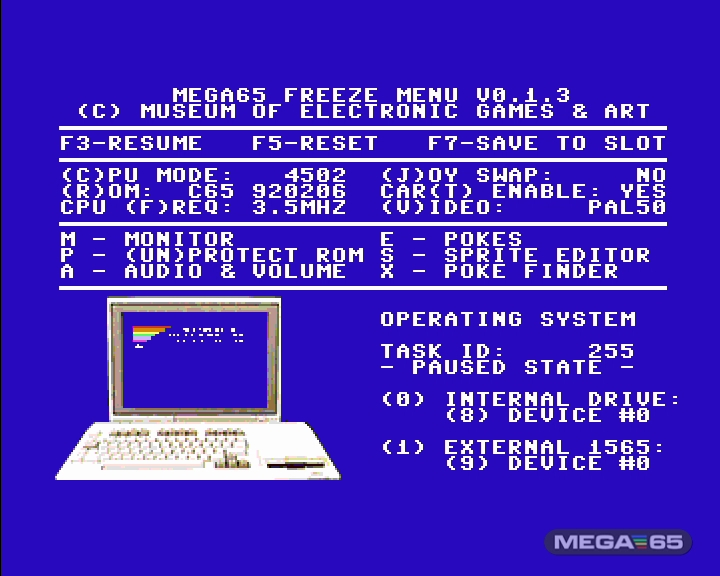
\includegraphics[trim= 10mm 20mm 10mm 20mm,clip,width=0.7\linewidth]{images/freezer.jpg}
\end{center}

\section{Terminology}

{\bf BASIC} and {\bf CBDOS} use following terminology:

{\bf UNIT} is a device number in the range 0-31.
The numbers from 0 to 11 are reserved for following device types:

{\ttfamily
\setlength{\tabcolsep}{1mm}
\begin{center}
\begin{tabular}{|l|l|l|}
\hline
 unit \# & device  & comment \\
\hline
0        & KEYBOARD & input \\
1        & unused   & was TAPE on C64 \\
2        & unused   & was RS232 on C64 \\
3        & SCREEN   & input/output     \\
4-5      & IEC PRINTER  & output     \\
6-7      & IEC PLOTTER  & output     \\
8-9      & CBDOS drives & floppy drive or disk image \\
10-11    & IEC drives   & 1541, 1571, 1581, FD-2000 \\
\hline
\end{tabular}
\end{center}
}

{\bf DRIVE} is the drive number inside a {\bf UNIT}.

{\ttfamily
\setlength{\tabcolsep}{1mm}
\begin{center}
\begin{tabular}{|l|l|l|}
\hline
 device  & drive numbers & comment \\
\hline
1581 IEC & 0             & single drive \\
1571 IEC & 0             & single drive \\
1541 IEC & 0             & single drive \\
FD-2000 IEC & 0             & single drive (CMD)\\
FD-4000 IEC & 0             & single drive (CMD)\\
SD2IEC      & 0             & drive images\\
\hline
\end{tabular}
\end{center}
}

For all single drives the drive number is always 0.
These are all known drives with an IEC interface, for example
the CBM drives 1541, 1571, 1581 and the CMD drives FD-2000 and FD-4000.
Also SD2IEC devices, which emulate a CBM drive using disk images on
SD-card.

Dual disk drives like 4040, 8050, 8250 which use drive numbers
0 and 1 are equipped with the IEEE-488 interface and need
an IEEE-488 to IEC converter to be used on the MEGA65.

The internal floppy controller of the MEGA65 can control
two floppy drives (one internal and one external, both attached to the same
ribbon cable). The {\bf FREEZER} can be used to assign D81 images from the
SD-card to the drive numbers 0 and/or 1, instead of physical floppy drives.

BASIC commands, that address files or disks, use therefore
{\bf U} for UNIT and {\bf D} for drive.
The default settings are {\bf UNIT = 8} and {\bf DRIVE = 0}.

\section{The Freezer}
The {\bf freezer} is a tool for changing system parameters at any time
regardless of the currently running program. The {\bf freezer} is invoked
by pressing \widekey{RESTORE} for approximately half to one second.
The current status of the computer is frozen and the freezer menu,
similar to the picture above, is displayed.
Most options are self explaining or will be covered in detail in the
online documentation. This chapter describes, how to assign disk images
and the internal floppy disk drive.

The bottom/right region of the freezer screen shows the current assignments.
The internal CBDOS (Computer Based Disk Operating System) can handle two
3.5" floppydrives or D81 images.
Drive 0 can be either the internal floppy disk drive or a D81 disk image.
Drive 1 can be either an external floppy disk drive (connected with the
same ribbon cable as the internal drive) or a D81 disk image.

The typical configurations will probably be:

Drive 0 :internal floppy disk drive, drive 1: disk image \\
Drive 0 :disk image, drive 1: disk image

The assignment, and the mounting of disk images can be done by pressing
\megakey{O} for drive 0 or \megakey{1} for drive 1.

The drive numbers are used internally by the CBDOS. BASIC and Kernal
however address the storage devices by {\bf UNIT} numbers.
The CBDOS fakes two single drives for the
operating system, by assigning separate unit numbers to drive 0 and drive 1.
The default assignment is:

{\bf UNIT 8, DRIVE 0} :internal drive 0 (internal floppy or disk image) \\
{\bf UNIT 9, DRIVE 0} :internal drive 1 (external floppy or disk image)

Sometimes one wants to change this unit assignment, if for example
a floppy drive 1541 is plugged in as unit 8 to the IEC port.
Then the internal drive assignment can be switched to an alternative unit
number, to avoid conflict.

\megakey{8} toggles the unit assignment of drive 0 between 8 and 10. \\
\megakey{9} toggles the unit assignment of drive 1 between 9 and 11.

After setting the preferences, the {\bf freezer} can be exited
with \megakey{F3}. The {\bf freezer} restores the screen and
returns to the interrupted program.

The drive and unit assignments are temporary and will be reset to default
after power down or reset. For permanent settings use the {\bf CONFIGURE}
menu.

